% Created 2022-01-14 Fri 12:54
% Intended LaTeX compiler: pdflatex
\documentclass[12pt]{article}
\usepackage[utf8]{inputenc}
\usepackage[T1]{fontenc}
\usepackage{graphicx}
\usepackage{longtable}
\usepackage{wrapfig}
\usepackage{rotating}
\usepackage[normalem]{ulem}
\usepackage{amsmath}
\usepackage{amssymb}
\usepackage{capt-of}
\usepackage{hyperref}
\usepackage{abntex2cite}
\usepackage[T1]{fontenc}		% Selecao de codigos de fonte.
\usepackage[utf8]{inputenc}		% Codificacao do documento (conversão automática dos acentos)
\usepackage{microtype} 			% para melhorias de
\RequireXeTeX %Force XeTeX check
\usepackage{xltxtra}
\usepackage{fontspec} %Font package
\newfontfamily\ch[Mapping=tex-text]{Noto Serif CJK TC}
\DeclareTextFontCommand{\unifont}{\ch}
\author{Pedro G. Branquinho, Wei-Liang Qian (\ch{钱卫良})}
\date{17 December 2021}
\title{Simulation and Modeling of Traffic Congestion.}
\hypersetup{
 pdfauthor={Pedro G. Branquinho, Wei-Liang Qian (\ch{钱卫良})},
 pdftitle={Simulation and Modeling of Traffic Congestion.},
 pdfkeywords={},
 pdfsubject={},
 pdfcreator={Emacs 27.2 (Org mode 9.6)}, 
 pdflang={English}}
\begin{document}

\maketitle
\tableofcontents

\clearpage
\section{Abstract}
\label{sec:org0433570}

We reproduced numerical method algorithms in this research. The initial
aim was at studying partial differential equations and to
recreate the simulations of a well known work on \emph{Traffic Flow} \cite{kerner1993}. Although the end goal was not achieved, the
research provided knowledge on the topics of \emph{Numerical Stiffness} and
the limitations of \emph{Physics Informed Neural Network} (PINN).

\section{Introduction}
\label{sec:orga5bbc5f}

Throughout the research, we used a \texttt{Version Control System} to keep a backup and
to track the progress; git and GitHub. The language chosen to model and compute
the PDEs was \texttt{Julia} \ref{sec:num-julia}.

The numerical methods explored consisted of Numerical
Analysis (von Neumman) \cite{press1986numerical}, Forward methods, and \texttt{Physics
Informed Neural Network} (PINN) \cite{zubov2021neuralpde}.

When the PINN method wasn't sufficient to solve the problem, a study about
\texttt{Numerical Stiffness} and the analytical numerical analysis became the focus of
the study. At this point, one of the programs developed dialed with simulating
\texttt{Stability Regions} of numerical methods \footnote{the program was based on \url{https://github.com/jverzani/ImplicitEquations.jl}}.

The equations we intended to simulate are a \texttt{non-linear system} \ref{sec:non-linear}.

\subsection{Analytical standpoint}
\label{sec:org5f3a230}
From a \emph{Analytical} point of view, Partial Differential Equations
(PDEs) differs from Ordinary Differential Equations (ODEs) in the
number of free variables. This means, in the case of PDEs the model depends on a
relationship of many variables and ODEs of only one.

\subsubsection{Definition}
\label{sec:orgb7d42a6}
A \texttt{partial differential equation} means a relation, for a given function
\texttt{u(x,y,...)} \cite{john1978partial},
\begin{equation}
\label{eq:PDE}
\begin{aligned}
F(x,y,\ldots ,u,u_{x}, u_{y}, \ldots, u_{xx}, u_{xy}, \ldots{})=0
\end{aligned}
\end{equation}

If more than one partial differential equation is needed to describe a model,
then these PDEs are called a \texttt{system}.

If substituted an \(u(\mathbf{x})\) which satisfies
\(F(\mathbf{x},\mathbf{u(x)})=0\). Then, \texttt{u} is a solution of the \texttt{PDE} or the
\texttt{system}.

\subsection{Numerical standpoint}
\label{sec:org36ed4fa}
The similarity between ODEs and PDEs, from a \emph{Numerical} point of view, is
that different approximation methods will result in different errors,
in relation to the exact, analytical, solution of the equations.

The need for numerical methods also unite both types of
equation. Since, even with ODEs as simple as the one derived from the
\emph{Simple Pendulum} do not have an analytical solution, without making simplifying
hypothesis \cite{brauer1989qualitative}.

\subsection{Methods studied}
\label{sec:orgf7e6c65}

\subsubsection{Ordinary Differential Equation}
\label{sec:orgf30f7a4}
Euler Forward, Backward and Adams-Moulton (trapezoidal) methods have been
studied with the standard test equation,

\begin{equation}
\begin{aligned}
y'(t)=e^{- \lambda{}t}
\end{aligned}
\end{equation}

This was done in other to both get used implementing numerical methods, and get
a better empirical sense of how different methods affect the accuracy of the
model.

Different variations of this system was simulated, in order to understand the
concepts of \texttt{Stiffness}, \texttt{A-stability} and \texttt{L-stability}.

\subsubsection{Nth-order methods for partial differentiation}
\label{sec:orgbace7c4}
The numerical methods were further explored using the analytical derivation of
higher order numerical formulas. These derivations consisting in using Taylor
Series and arrive at a formula considering \texttt{n} points to calculate a step. E.g.,
for the second order partial differential of the third order

\begin{equation}
\begin{aligned}
\dfrac{\partial^2{u}}{\partial{x^2}}\biggr\rvert_i = \dfrac{u_{i+1}-2u_i+u_{i-1}}{\Delta{x^2}} - O(\Delta{x^2})
\end{aligned}
\end{equation}

\subsection{Analytical theory on perturbations}
\label{sec:org043d0f9}
On Kerner's paper, he uses perturbation theory to developed the analytical
formulas that implies the existence of a clustering effect - traffic jams - even
with extremely initial small perturbations \cite{kerner1993}.

In order to better understand these derivations, material has been studied on
the topic \cite{tremblay2017phy}, and a derivation of the spring-mass equations for a small pertubation
was derived.

\section{Bibliography Review}
\label{sec:orgb94241a}
\subsection{Development of the field}
\label{sec:orgb55d75d}
\subsubsection{The dawn of numerical methods}
\label{sec:org8f253cb}
Numerical analysis dawn can be dated to
1820 B.C. \cite{smith1930rhind}, with Egyptian's methods for
calculating roots.

Although, modern methods for solving ODEs and PDEs were mainly
developed after the discovery of \emph{Calculus}, in the 17th century.

\subsubsection{Modern methods and Computing}
\label{sec:orgfd71f3e}
Currently, even though sophisticated mathematics has been
developed to accurately simulate virtually any ODE, the mathematics
for solving PDEs is still a open field. This is due to the nature of
PDEs which do not have a general method or procedure that is
efficient, when simulating them.

\subsubsection{Physics Informed Neural Networks}
\label{sec:org420448b}
There exists methods aimed at using the computational power available in computers
to abstract the theoretical knowledge of Numerical Stability away from
the problem. \emph{Physics Informed Neural Network}
(PINN) is one of these methods. The shortcoming of the method is the loss of the
possibility of making small adjustments to the resulting \emph{Numerical
Method}, as will be discussed further on the results.

\subsubsection{Numerical Instability}
\label{sec:org323599d}
Each equation, and it's constant parameters, will have specific method
or a coupling of methods suited to the simulation of a PDE.

\subsubsection{Grouping of methods and types of PDEs}
\label{sec:org601ed5d}
Broadly, methods are associated with the kind of partial differential
equation one is studying. These equations can be either \texttt{Hyperbolic},
\texttt{Parabolic} or \texttt{Elliptic}. Also, equations can be mixed, e.g., \texttt{Mixed
Parabolic-Hyperbolic}, etc.

\subsection{Mathematical categorization of PDEs}
\label{sec:org555a840}
\subsubsection{Order of equations and systems}
\label{sec:orgffa886a}
``The order of the system is the order of the highest derivative that occurs.''
\cite{john1978partial}. In which, irrespective of the free variable, we count the
total number of derivatives. E.g., a sixth order equation, with mixed variables.

\begin{equation}
\label{eq:sixth-order}
\begin{aligned}
F(\mathbf{x},\mathbf{u(x)}) = 0 \, \land \,
F(\mathbf{x}) = \dfrac{\partial{}^6 \mathbf{u}}{(\partial{x})^2(\partial{y})^2(\partial{z})} + \dfrac{\partial^3{} \mathbf{u}}{(\partial{x})^3}
\end{aligned}
\end{equation}

\subsubsection{Linearity, quasi-linearity and non-linearity}
\label{sec:org78c774f}
\begin{enumerate}
\item Linearity
\label{sec:orge8c4e5f}

Linearity is defined as not having any term in the \eqref{eq:PDE}, such that it's
a result of a multiplication of two independent terms. The independent terms
being \(\mathbf{x}\), \(u(\mathbf{x})\) and all partial derivatives of
\(u(\mathbf{x})\).

For example, the second order linear equation with constant
coefficients, \texttt{Kolmogorov's equation} \cite{evans1998partial},
\begin{equation}
\begin{aligned}
u_{t} - \sum_{i,j=1}^{n}{a^{ij}u_{x_{i}x_{j}}} + \sum_{i}^{n}{b^{i}u_{x_{i}}} = 0
\end{aligned}
\end{equation}

We see there is no non-linear terms, as the product \(u_{x_{i}}*u_{x_{j}}\), etc.

\item Non-linear equations
\label{sec:org5fe54f7}
\label{sec:non-linear}

The physical model we are interested deals with an equation similar to the
\texttt{Navier-Stokes} equation \cite{kerner1993}. The \texttt{Navier-Stokes} equations are a
nonlinear system \cite{john1978partial} \cite{kerner1993}.
E.i.,

\begin{equation}
\label{eq:NavEstEQ}
\begin{aligned}
\begin{cases}
&\mathbf{u}_t + \mathbf{u} \cdot{} D\mathbf{u} - \nabla \mathbf{u} = - Dp \\
&\text{div}(\mathbf{u}) = 0
\end{cases}
\end{aligned}
\end{equation}

\item Quasi-linear equations
\label{sec:org582f9ae}

A special kind of equations that follow under the category of non-linear
equations are the quasi-linear equations. These have the non-linear terms which
are of a lesser order than the order of the equation. E.g., the \texttt{Korteweg-de
Vries} equation \cite{john1978partial},

\begin{equation}
\begin{aligned}
u_t + c uu_{x} + u_{xxx} = 0
\end{aligned}
\end{equation}
\end{enumerate}

\subsubsection{Elliptic, hyperbolic and parabolic PDEs}
\label{sec:org9046ac6}
Given the general quasi-linear equation for a function \texttt{u},

\begin{equation}
\label{eq:general-2th-order}
\begin{aligned}
au_{xx} + 2bu_{xy} + cu_{yy} = d
\end{aligned}
\end{equation}

where \(a\), \(b\), \(c\) and \(d\) are of the form \(f(x,y,u,u_x,u_y)\).

We can develop an analysis of how the solution would behave. \emph{A priori}, the
solution \(\gamma\) is contained on the xy-plane.

From this consideration, if carried an analysis on the curve itself, we
ultimately arise at the condition:

\begin{equation}
\begin{aligned}
\dfrac{dy}{dx} = \dfrac{b \pm \sqrt{b^2 -ac}}{a}
\end{aligned}
\end{equation}

Then, if \(ac-b^2>0\) it's \texttt{elliptic}; else, if \(ac-b^2<0\) it's called
\texttt{hyperbolic}. Finally, if \(ac-b^2=0\) we call it \texttt{parabolic}.

These categories help understand the expected behavior of the solution. But, in
nonlinear cases the PDE do not characterize the solution behavior in these
categories; and in some linear cases, different regions will have different
types of behaviors, regarding the \texttt{elliptic}, \texttt{hyperbolic} and \texttt{parabolic}
characterization \cite{john1978partial}.

\subsection{Numerical Methods implemented in Julia}
\label{sec:org06a2eb4}
\label{sec:num-julia}

There exists a variety of libraries on \emph{numerical methods}
available in modern languages. Most of them with ports of libraries
written in C and FORTRAN. To list a few, from the \texttt{Julia}
documentation on available methods:

\begin{itemize}
\item General PDE approximation methods.
\item Transform methods.
\item Finite difference methods.
\item Finite element methods.
\item Finite volume methods.
\item Spectral element methods.
\item Boundary element, Boundary integral methods.
\item Mesh free methods and particle methods.
\item Virtual element methods.
\item Multi-method packages.
\item Non-classical methods.

\textbf{Source:} \url{https://github.com/JuliaPDE/SurveyofPDEPackages}
\end{itemize}
\subsection{{\bfseries\sffamily TODO} PINN}
\label{sec:org8c9ff59}

Physics Informed Neural Networks

\section{Materials and Methods}
\label{sec:org6920671}

The materials used were:
\begin{itemize}
\item Git
\item GitHub
\item Julia language
\end{itemize}

\subsection{{\bfseries\sffamily TODO} Version Control}
\label{sec:org690609a}
\subsection{{\bfseries\sffamily TODO} Julia language}
\label{sec:org412a699}
\subsection{{\bfseries\sffamily TODO} PINNs}
\label{sec:orgfd82340}
\subsection{{\bfseries\sffamily TODO} Developed code}
\label{sec:org86f9dd4}
\subsection{{\bfseries\sffamily TODO} Stability Regions}
\label{sec:orgb071807}
\section{Results and Discussion}
\label{sec:orga9122c5}
\subsection{{\bfseries\sffamily TODO} Kerner's reproduction through PINNs}
\label{sec:org14ffb3d}

\begin{figure}[!htb]
  \centering
  \caption{\label{fig:sim1} Reproduction try, using PINN. Source: The authors}
  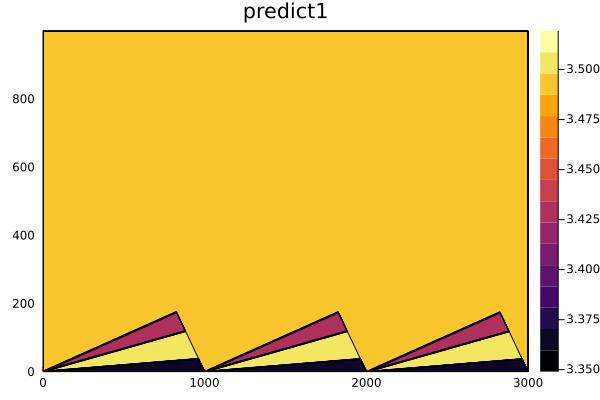
\includegraphics[width=0.45\linewidth]{../img/sol_variable_corrected_bcs31.png}
  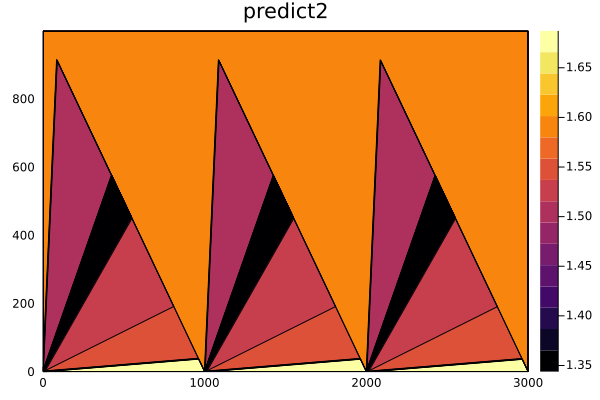
\includegraphics[width=0.45\linewidth]{../img/sol_variable_corrected_bcs32.png}
  \\ %\legend{}
\end{figure}
\clearpage

\begin{figure}[!htb]
  \centering
  \caption{\label{fig:sim2} Original simulation. Source: Image from Kerner and Konhäuser \cite{kerner1993}}
  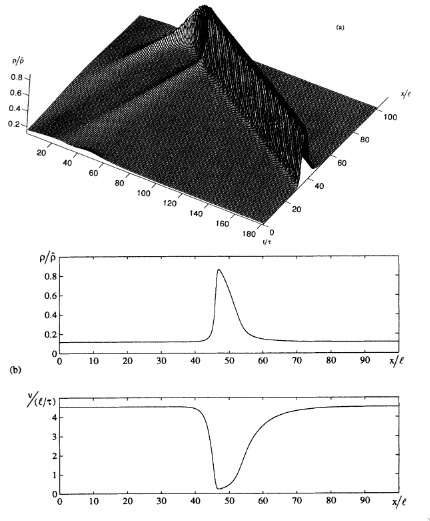
\includegraphics[width=0.4\linewidth]{./resources/kerner.png}
  \\  %\legend{Fonte: Imagem de Kerner e Konhäuser \cite{kerner1993cluster}}
\end{figure}
\subsection{{\bfseries\sffamily TODO} Steps to derive the Stability Region}
\label{sec:org15fb6e0}
\subsection{{\bfseries\sffamily TODO} Stiffness}
\label{sec:orgfbdd1ef}
\subsection{Nth-order approximation}
\label{sec:orga0598aa}
\subsubsection{Third-order approximation of second-order differential equation}
\label{sec:org8357717}

By Taylor Expansion
\begin{equation}
\begin{aligned}
\begin{cases}
u_{i+1} &= u_{i} + \Delta{x}\dfrac{\partial{u}}{\partial{x}}\biggr\rvert_i + \dfrac{\Delta{x^2}}{2!}\dfrac{\partial^2{u}}{\partial{x^2}} + \ldots \\
u_{i-1} &= u_{i} - \Delta{x}\dfrac{\partial{u}}{\partial{x}}\biggr\rvert_i + \dfrac{\Delta{x^2}}{2!}\dfrac{\partial^2{u}}{\partial{x^2}} + \ldots
\end{cases}\\
\sim
\begin{cases}
u_{i+1} &= u_{i} + \sum_{n=1}^{M}{\dfrac{(\Delta{x})^n}{n!}\dfrac{\partial^n{u(x)}}{\partial{x^n}}\biggr\rvert_i}\\
u_{i-1} &= u_{i} + \sum_{n=1}^{M}{(-1)^n\dfrac{(\Delta{x})^n}{n!}\dfrac{\partial^n{u(x)}}{\partial{x^n}}\biggr\rvert_i}
\end{cases}
\end{aligned}
\end{equation}

Summing both terms and isolating
\(\dfrac{\partial^2{u}}{\partial{x^2}}\biggr\rvert_i\), we have:

\begin{equation}
\begin{aligned}
\dfrac{\partial^2{u}}{\partial{x^2}}\biggr\rvert_i = \dfrac{u_{i+1}-2u_i+u_{i-1}}{\Delta{x^2}} - O(\Delta{x^2})
\end{aligned}
\end{equation}

\section{Conclusion}
\label{sec:org79e9334}
The use of PINNs got us closer to reproducing Kerner's
results. But, at the same time, the pigtail of using a method that
hide us the ability of adjusting the discretization showed itself,
once the results were not satisfactory.

After getting stuck on this riddle, we took the path of learning more
about \emph{classical methods} on numerical methods for PDEs. Knowledge on
the subject of \emph{equation Stiffness} was gained in the process e.g., why
and how to categorize methods and to grasp what does it mean to an
equation to be stiff.

\bibliography{../../../Bibliography/collection}
\end{document}
